\documentclass[14pt]{mmcs_article}
\usepackage[russian]{babel}
\usepackage{amsmath, amsthm, amsfonts, amssymb}
\usepackage{tikz}
\usetikzlibrary{positioning}

\newenvironment{myitemize}
{ \begin{itemize}
		\setlength{\itemsep}{0pt}
		\setlength{\parskip}{0pt}
		\setlength{\parsep}{0pt}     }
	{ \end{itemize}                  } 

\newenvironment{myenumerate}
{ \begin{enumerate}
		\setlength{\itemsep}{0pt}
		\setlength{\parskip}{0pt}
		\setlength{\parsep}{0pt}     }
	{ \end{enumerate}                  } 

%\graphicspath{{images/}}%путь к рисункам

\begin{document}

% Титульные листы
% раскомментировать требуемое
%%см. РЕКОМЕНДАЦИИ ПО ОФОРМЛЕНИЮ
%И ПРЕДСТАВЛЕНИЮ КУРСОВЫХ И ВЫПУСКНЫХ %КВАЛИФИКАЦИОННЫХ РАБОТ СТУДЕНТОВ ИНСТИТУТА %МАТЕМАТИКИ, МЕХАНИКИ И КОМПЬЮТЕРНЫХ НАУК


% ----------------------------------
% Внимание!
% Изменяйте только строки, перед которыми стоят знаки комментариев
% ----------------------------------

\thispagestyle{empty}
\begin{singlespacing}
\begin{center}

МИНОБРНАУКИ РОССИИ\\ [12pt]
Федеральное государственное автономное образовательное\\
учреждение высшего образования\\
<<Южный федеральный университет>>

\vspace{\baselineskip}
Институт математики, механики\\
и компьютерных наук им.~И.\,И.~Воровича

\vspace{\baselineskip}
% Название выпускающей кафедры
Кафедра алгебры и дискретной математики

\vfill
% Фамилия Имя Отчество студента
\textbf{Иванов Сергей Иванович}

\vspace{\baselineskip}
%%НАЗВАНИЕ РАБОТЫ должно полностью соответствовать распоряжению по Институту (для курсовых работ).
{\bf НАЗВАНИЕ РАБОТЫ, \\
РАЗБИТОЕ ПРИ НЕОБХОДИМОСТИ \\
НА НЕСКОЛЬКО СТРОК }

\vspace{15mm}
КУРСОВАЯ РАБОТА\\
по направлению подготовки\\
% указать направление обучения (раскомментируйте нужную строчку)
01.03.02~-- Прикладная математика и информатика
% 01.03.01~-- Математика
% 01.03.03~-- Механика и математическое моделирование 	
% 02.03.02~-- Фундаментальная информатика и информационные технологии


\vspace{10mm}
\textbf{Научный руководитель~--}\\
% указать данные о руководителе
% должность, степень, звание Фамилия Имя Отчество
проф., д.\,ф.-м.\,н. Сергеев Петр Сергеевич

\vspace{20mm}

\noindent
\begin{flushleft}
$\overline{\textrm{оценка (рейтинг)}}$\qquad	$\overline{\textrm{подпись руководителя\vphantom{й}}}$

\end{flushleft}


\vfill
% год!
Ростов-на-Дону -- 2020

\end{center}

\singlespacing
\end{singlespacing}  % для курсовой
%%см. РЕКОМЕНДАЦИИ ПО ОФОРМЛЕНИЮ
%И ПРЕДСТАВЛЕНИЮ КУРСОВЫХ И ВЫПУСКНЫХ %КВАЛИФИКАЦИОННЫХ РАБОТ СТУДЕНТОВ ИНСТИТУТА %МАТЕМАТИКИ, МЕХАНИКИ И КОМПЬЮТЕРНЫХ НАУК


% ----------------------------------
% Внимание!
% Изменяйте только строки, перед которыми стоят знаки комментариев
% ----------------------------------

\thispagestyle{empty}
\begin{singlespacing}
\begin{center}

МИНОБРНАУКИ РОССИИ\\ [12pt]
Федеральное государственное автономное образовательное\\
учреждение высшего образования\\
<<Южный федеральный университет>>

\vspace{\baselineskip}
Институт математики, механики\\
и компьютерных наук им.~И.\,И.~Воровича

\vspace{\baselineskip}
% Название выпускающей кафедры
Кафедра алгебры и дискретной математики

\vfill
% Фамилия Имя Отчество студента
\textbf{Иванов Иван Сергеевич}

\vspace{\baselineskip}
%НАЗВАНИЕ РАБОТЫ должно полностью соответствовать
% приказу по ЮФУ (для выпускных квалификационных работ)
{\bf НАЗВАНИЕ РАБОТЫ, \\
РАЗБИТОЕ ПРИ НЕОБХОДИМОСТИ \\
НА НЕСКОЛЬКО СТРОК }

\vspace{15mm}
ВЫПУСКНАЯ КВАЛИФИКАЦИОННАЯ РАБОТА\\
по направлению подготовки\\
% Направление обучения
% раскомментируйте нужную строчку
02.03.02~-- Фундаментальная информатика и информационные технологии
% 01.03.01~-- Математика
% 01.03.02~-- Прикладная математика и информатика
% 01.03.03~-- Механика и математическое моделирование 	


\vspace{10mm}
\textbf{Научный руководитель~--}\\
% указать данные о руководителе
% должность, степень, звание Фамилия Имя Отчество
проф., д.\,ф.-м.\,н. Сергеев Петр Сергеевич

\vspace{15mm}

\noindent
% указать Фамилию и инициалы 
% заведующего выпускающей кафедры
\begin{flushleft}
Допущено к защите:\\
заведующий кафедрой \underline{\hspace*{65mm}} Сидоров С.\,С.
\end{flushleft}




\vfill
% год!
Ростов-на-Дону -- 2020

\end{center}

\singlespacing
\end{singlespacing} % для работы бакалавра
%см. РЕКОМЕНДАЦИИ ПО ОФОРМЛЕНИЮ
%И ПРЕДСТАВЛЕНИЮ КУРСОВЫХ И ВЫПУСКНЫХ %КВАЛИФИКАЦИОННЫХ РАБОТ СТУДЕНТОВ ИНСТИТУТА %МАТЕМАТИКИ, МЕХАНИКИ И КОМПЬЮТЕРНЫХ НАУК


% ----------------------------------
% Внимание!
% Изменяйте только строки, перед которыми стоят знаки комментариев
% ----------------------------------

\thispagestyle{empty}
\begin{singlespacing} 
\begin{center}

МИНОБРНАУКИ РОССИИ\\ [12pt]
Федеральное государственное автономное образовательное\\
учреждение высшего образования\\
<<Южный федеральный университет>>

\vspace{\baselineskip}
Институт математики, механики\\
и компьютерных наук им.~И.\,И.~Воровича


\vfill
% Фамилия Имя Отчество студента
\textbf{Соколов Михаил Игоревич}

\vspace{15mm}
%НАЗВАНИЕ РАБОТЫ должно полностью соответствовать 
% приказу по ЮФУ (для выпускных квалификационных работ)
{\bf СОЗДАНИЕ МЕТА-РЕКОМЕНДАТЕЛЬНОЙ СИСТЕМЫ \\
ДЛЯ ИНТЕРНЕТ-МАГАЗИНОВ \\
НА ОСНОВЕ СУЩЕСТВУЮЩИХ МОДЕЛЕЙ }

\vspace{15mm}
ВЫПУСКНАЯ КВАЛИФИКАЦИОННАЯ РАБОТА\\
по направлению подготовки\\
% Направление обучения 
02.04.02~-- Фундаментальная Информатика и информационные технологии,\\
направленность программы\\
<<Математическое и программное обеспечение вычислительных машин>>

\vspace{10mm}
\textbf{Научный руководитель~--}\\
% указать данные о руководителе
% должность, степень, звание Фамилия Имя Отчество
доц., к.\,т.\,н. Чердынцева Марина Игорьевна

\vspace{7mm}
\textbf{Рецензент~--}\\
% указать данные о рецензенте
% должность, степень, звание Фамилия Имя Отчество
к.\,т.\,н. Штейнберг Роман Борисович 


\vspace{15mm}

\noindent
% указать Фамилию и инициалы руководителя
% образовательной программы
\begin{flushleft}
Допущено к защите:\\
руководитель \\
образовательной программы \underline{\hspace*{64mm}} Фёдорова Я.\,М.
\end{flushleft}




\vfill
% год!
Ростов-на-Дону -- 2022

\end{center} 

\singlespacing
\end{singlespacing}% для работы магистра

\renewcommand{\contentsname}{Оглавление}

\tableofcontents

%=======================
\newpage
\addcontentsline{toc}{section}{Постановка задачи}

\section*{Постановка задачи}


Цель работы - создание мета-рекомендательной системы, способной адаптироваться и давать рекомендации для любого интернет-магазина. Для достижения цели был сформирован набор рабочих задач:
\begin{enumerate}
	\item Анализ полученных из интернет-магазинов треков активности пользователей и описания продаваемых товаров
	\item Выбор методов рекомендации, подбор типов моделей-рекомендаторов.
	\item Формирование представлений данных для создания и обучения моделей.
	\item Обучение моделей и поиск оптимальных гиперпараметров.
	\item Добавление возможности автоматического пересоздания представлений данных и моделей и переобучения моделей в связи с изменившимися данными и возможности использования оперативной истории без переобучения моделей
	\item Интеграция в существующую платформу интернет-магазинов.
\end{enumerate}

Для решения задачи( по согласованию с заказчиком) был выбран ЯП Python с пакетами numpy v 1.19.5, scikit-learn v 1.0.0, scipy v 1.7.1, implicit v 0.4.4, pandas v 1.3.5 и TensorFlow v 2.4.2, а также использовался NVidia CUDA Toolkit v 10.1 для ускорения обучения определенных нейросетевых моделей с использованием GPU.

В дальнейшем может быть апдейтнем версию TensorFlow до 2.7.*... Но пока нет. 


%=======================
\newpage
\addcontentsline{toc}{section}{Введение}
\section*{Введение}

Дальнейшее повышение эффективности работы субьектов электронной коммерции, на наш взгляд, связано с расширением списков клиентов, получающих доступ к упомянутым субьектам. В данном отчете описана попытка создания решения на базе собранной информации интернет-магазинов. \\
Эта работа может быть использована в предприятих электронной коммерции (интернет-магазинах) для быстрого и легкого создания и обновления автоматической рекомендательной системы и соответственно, имеет высокую практическую значимость.
Результаты данной работы апробированы на конференции "Математика. Компьютер. Образование. 2022".

%=======================
\newpage
\section{Входные данные. EDA}\label{dsfs}
Заказчиком были предоставлены экземпляры файлов, выгружаемых с с интернет-магазинов. 
Файл 1 типа - .csv  файл, содержащий описание событий происходящих в интернет-магазине, в дальнейшем - данные о событиях. \\
Всего файл 1 типа содержит 44 типа полей, однако некоторые из них не заполнены во всем датасете. Далее следует список полей и гипотез для каждого поля. Незаполненные поля, а также поля не несущие полезной информации(сервисные хеши и т.д) опущены.
\begin{myenumerate}
	\item datetime. Поле времени начала события. 
	\item userip. Поле, в котором указывается IPv4-адрес, с которого осуществлялся доступ. Гипотеза: можно использовать для генерации рекомендаций по стране пользователя.
	\item userid. Цифробуквенный уникальный ID пользователя в системе, основной способ идентификации пользователя.
	\item useragent. Фрагмент HTML-header, указывающий на используемый браузер. Гипотеза: можно использовать тип браузера для дифференциации положения владельца в обществе.
	\item eventtype. Тип произошедшего события. 
	\begin{myenumerate}
		\item ProductView - события просмотра товара пользователем. 
		\item AddToCart - события добавления пользователем товара в корзину. 
		\item FacetSelection - событие выбора пользователем фильтра показа товаров.  
		\item Search - событие поиска пользователем товара по названию.
		\item AutoComplete - событие автодополнения запроса пользователя. 
		\item ClickOnSearchResult - событие нажатия на результат поисковой выдачи. 
	\end{myenumerate}
	\item usersearchphrase Запрос пользователя. Используется в типах событий AutoComplete, Search. Гипотеза: Может быть использовано для лингвистического анализа запроса.
	\item correctedsearchphrase. Исправленный запрос пользователя. Используется в типе событий Search. 
	\item facetname. Имя фильтра по которому производился поиск. Используется в типе событий Facet Selection. 
	\item facetvalue. Значение фильтра. Используется в типе событий Facet Selection. Гипотеза: может быть использовано при рекомендации, отфильтровывая рекомендации по соответствующему значению. 
	\item productid. Внутренний уникальный ID продукта. 
\end{myenumerate}

Файл 2 типа - .json файл содержащий описания товаров, а также фильтров товаров, представленных в магазине. Вследствие предполагаемой универсальности системы, а также большого количества полей, являющимися пустыми, приведем описание только используемых универсальных полей, и обобщенное описание остальных полей.\\
В данном файле интерес представляют два поля: Items и Facets. Рассмотрим их подробнее. \\
Поле Items:
\begin{myenumerate}
	
	\item CatalogID. Уникальный числовой ID продукта. Совпадает со значением поля productid в событиях типа ProductView.
	\item Name. Имя товара. Гипотеза: может быть использовано для поиска похожих по названию товаров.
 	\item OrdersCount. Количество заказанных товаров. Гипотеза: можно использовать для фильтрации товаров по популярности.
	\item Типы и значения фильтров, отвечающих товару.
\end{myenumerate}

Поле Facets:
\begin{myenumerate}
	
	\item FacetName. Имя фильтра.
	\item TotalHits. Количество раз, который этот фильтр был выбран. Гипотеза: Может быть использовано для определения самых часто выбираемых фильтров.
	\item Values. Список возможных значений, которые может принимать фильтр. Может иметь как категориальный тип, так и числовой тип. 
\end{myenumerate}

После проведенного EDA, было принято решения использовать лишь следующие поля:

Из файлов 1 типа(событий):

\begin{myenumerate}
		\item datetime.
		\item userid. 
		\item productid.
		\item eventtype. Было принято решение для простоты использовать исключительно типы событий ProductView и AddToCart, так как они несут наибольшее количество полезной информации для рекомендательной системы. 
\end{myenumerate}

Из файлов 2 типа(предметов):

\begin{myenumerate}
	\item CatalogID.
	\item Типы и значения фильтров, отвечающих товару
\end{myenumerate}

Кроме того, такой подход позволяет значительно сократить количество используемой ОЗУ и памяти для хранения данных.

Для обработки данных был создан специализированный пайплайн. Он состоит из 6 стадий обработки данных, которые можно представить в виде следующего графа.

\begin{figure}[H]
\begin{tikzpicture}[main/.style = {draw, rectangle},node distance= 1cm,align=left] 
\node[main] (1) {prepare\_actions(1)}; 
\node[main] (2) [below=0.5cm of 1] {prepare\_df\_splits(2)};
\node[main] (3) [below left=0.5cm and -1cm of 2] {prepare\_csr\_splits(3)}; 
\node[main] (4) [below right=0.5cm and -2cm of 2] {prepare\_items\_by\_users(4)}; 
\node[main] (5) [right=1cm of 1] {prepare\_item\_profiles(5)}; 
\node[main] (6) [below right=0.5cm and -2cm of 4] {prepare\_user\_profiles(6)}; 
\draw[->] (1) -- (2);
\draw[->] (2) -- (3);
\draw[->] (2) -- (4);
\draw[->] (4) -- (6);
\draw[->] (5) -- (6);
\end{tikzpicture}
\caption{Граф пайплайна системы}\label{stud:fig:2}
\end{figure}
На каждом этапе формируется одно из представлений данных. Кратко опишем их.

\begin{myenumerate}
	\item Стадия prepare\_actions. На ней формируется временное представление - $pandas$.$dataframe$, содержаший в себе записи о всех событиях типа  ProductView и AddToCart.
	\item Стадия prepare\_df\_splits. На ней формируется основное представление данных, представляющее собой два  $pandas$.$dataframe$ - соответственно train и test. train содержит в себе все события, произошедшие до определенной даты включительно, test - все события, которые произошли после определенной даты. Важно, что test содержит в себе события только тех пользователей, которые входят во множество train. 
	\item Стадия prepare\_csr\_splits. На ней, на основе результатов стадии prepare\_df\_splits формируются два основных представления данных CSR(csr\_train и csr\_test) - разреженные матрицы формата \\$scipy$.$sparse$.$csr\_matrix$, содержащие все взаимодействия пользователей со всеми товарами(c повышающими коэффициентами для событий AddToCart). Так, одно событие AddToCart рассматривается как одно или более событий ProductView - конкретный коэффициент задается в конфигурационном файле системы. Путем экспериментов, был подобран коэффициент = 10.
	\item Стадия prepare\_items\_by\_users. На этой стадии создается словарь взаимодействия userid и productid, что используется для контроля обучения моделей и в стадии prepare\_user\_profiles.
	\item Стадия prepare\_item\_profiles. На этой стадии формируется представление данных ItemProfileStorage - создается таблица(pandas.DataFrame), содержащая профили всех товаров, построенная на извлеченных из .json файла фильтров показа и их значений. Строки таблицы - товары, столбцы - характеристики товаров. 
	\item Стадия prepare\_user\_profiles. На этой стадии формируется представление данных UserProfileStorage - таблица(pandas.DataFrame), содержащая профили всех пользователей, построенная на извлеченных из .json файла фильтров показа и их значений и представлении данных IP. Каждый профиль пользователя представляет собой алгебраическую сумму профилей всех товаров, с которыми он взаимодействовал(точно так же, как в CSR - c повышающими коэффициентами для событий AddToCart). Это основа для собственного подхода, объединяющего принципы Content based подхода и коллаборативной фильтрации.
	
\end{myenumerate}

Основные представления данных, которые будут использованы в дальнейшем - CSR, ItemProfileStorage, UserProfileStorage.

%=======================

\section{Модели}\label{dsfs}
Далее были созданы одна модель - baseline и 6 моделей машинного обучения. Перечислим их по порядку: TopN, ALS, BPR, AE, IP, UIP, DRN. Выход каждой модели - список товаров, которые необходимо рекомендовать пользователю. \\
Стоит заметить, что процесс генерации и обучения моделей также является полностью автоматизированным, что позволяет переобучать модели без участия ml-инженеров. К сожалению, все модели(за исключением Top30) жестко привязываются к данным, что делает процесс дообучения на новых данных невозможным, вследствие чего используется процесс полного переобучения.
\subsection{TopN}
Самая очевидная и простая модель - любому пользователю предлагается N самых популярных товаров. Данная модель используется в качестве baseline для всех остальных моделей, а также для дополнения списка рекомендаций в случае если другие модели не смогли дать необходимое их число.
\subsection{ALS}
Модель ALS \cite{ALSA1}. Данная модель принадлежит к классу collaborative filtering. \\
Введем отношения, необходимые для работы данной модели. Пусть у нас есть m пользователей и n продуктов, предлагаемые им. Запишем все взаимодействия пользователей и продуктов в матрицу $R_{m \times n}$, где $R_{i,j}$ - количество раз которое пользователь $i$ взаимодействовал(в нашем случае просматривал) товар $j$. Результирующая матрица является разреженной. \\
ALS(Alternating Least Squares) это итеративный процесс факторизации матрицы $R$ на матрицы $U_{m \times k}$ и $V{k \times n}$ такие, что  $R \approx U^TV$. Здесь $k$ означает количество скрытых признаков.\\
Для нахождения матриц $U$, $V$ необходимо решить следующую оптимизационную задачу: 
\begin{equation}
argmin_{U,V} \sum_{(i,j|r_{i,j} != 0)} (r_{i,j} - U_i^TV_j)^2 + \lambda (\sum_i n_{u_i} {\parallel u_i \parallel} ^2 + \sum_j n_{v_j} {\parallel v_j \parallel} ^2) 
\end{equation}
Здесь $\lambda$ - сила регуляризации, $n_{u_i}$ - количество продуктов просмотренных пользователем $i$,  $n_{v_j}$ - количество раз, которые был просмотрен товар $j$. \\
Поочередно фиксируя матрицы $U$ и $V$, мы получаем квадратное уравнение, которое можно решить, и , таким образом, итеративно улучшить качество разложения. \\
Очевидно, что данная модель использует представление данных CSR. В качестве реализации данной модели была взята библиотека implicit \cite{ALSA2} для ЯП Python.
\\

%\subsection{BPR}
%Модель BPR также принадлежит к классу collaborative filtering. \\
%Для работы модели необходимы ровно те же отношения, что и для работы модели ALS. Внутри, впрочем данная %модель использует метод попарного ранжирования отношения пользователя $i$ к продуктам $j1$ и $j2$. 
%Данная модель также использует модель представления CSR.
\subsection{AE}
Модель AE(AutoEncoder) принадлежит к классу collaborative filtering. \\

Для работы модели необходима матрица взаимодействия пользователь-товар. Идея данного подхода заключается в том, чтобы С помощью нейронной сети предпринимается попытка восстановить строку матрицы взаимодействия пользователь-товар.\cite{AEA1} \\

Как известно, автоенкодер представляет собой нейронную сеть, выполняющую 2 преобразования  $encode(x) : Rn \rightarrow Rd$ и $decode(x) : Rd \rightarrow Rn$. Цель этих преобразований получить представление данных исходной размерности $n$ в размерности $d$ такую, чтобы минимизировать отклонение $x\_received =decode(encode(x))$.

Данная модель представляет собой достаточно простой автоенкодер. Енкодер представлен одним Dense Layer с размерностью входа(n) равной количеству товаров, и размерностью выхода(Bottleneck) экспериментально подобранной как 256(d). Декодер, соответственно, представлен одним DenseLayer с размерностью входа($d$) 256 и размерностью выхода ($n$) равной количеству товаров. 

Особо стоит отметить процесс выбора функций активации и loss-функции. Вследствие характера обрабатываемых данных(implicit feedback пользователей), нежелательна потеря отрицательных значений после активации, что делает нерациональным использование стандартного в таких случаях ReLU( Rectified Linear Unit). Поэтому в качестве функции используется ELU(Exponential Linear Unit). В дальнейшем будет произведен эксперимент с использованием SELU(Scaled Exponential Linear Unit).\\

В подобных задачах часто используют masked mse (loss оценивается только по не нулевым позициям входного вектора, позволяя сети сколько угодно сильно "ошибаться" по тем позциям, где стояли нули.) в качестве loss-функции.  Но при решении данной задачи этот метод не сработал. Обычный mse отлично справляется и не может занулить все наши рекомендации просто по тому, то автоэнкодер не может дать 100\% точность после разжатия данных.


\subsection{IP}
Модель IP является представителем item-based подхода. \\
Построенные в представлении данных IP профили товаров используются как обучающий dataset для модели sklearn.NearestNeighbours, имеющий в основе алгоритм KD-Tree. Данная модель позволяет как рекомендовать товары, похожие на данный, так и рекомендовать товары на основе истории пользователя.  
В случае рекомендаций товаров на основе истории взаимодействий пользователя, применяется следующий алгоритм:

Правило брать не более чем 3 похожих на текущий товара выведено экспериментально.
\subsection{UIP}
Аналогично, построенные в представлении данных UIP профили пользователей используются как обучающий dataset для модели sklearn.NearestNeighbours, имеющий в основе алгоритм KD-Tree. Данная модель позволяет находить пользователей, похожих на данного, и, соответственно, рекомендовать пользователю товары, являющиеся популярными у похожих пользователей.
Применяется следующий алгоритм:

Аналогично, правило брать не более чем 5 товаров у похожего пользователя выведено экспериментально.
\subsection{DRN}

Данная модель примечательна тем, что она является гибридной, совмещая в себе подходы collaborative filtering и content-based. Также, она примечательна и своей конструкцией - это сиамская нейронная сеть, имеющая структуру, приведенную ниже. Задача этой сети - обучиться отличать вещи которые могут понравиться пользователю. Необычен и процесс обучения - на вход данной модели подаются тройки вида (профиль пользователя, профиль понравившейся ему вещи, профиль не понравившейся ему вещи).

Данная модель использует две подмодели - для создания embedding товаров (Dense Layer размерности 64, ReLU, Dense Layer размерности 32, ReLU) и embedding пользователей (Dense Layer размерности 32, ReLU). Оба embedding передаются в ScoreLayer, где определяется близость embedding пользователя к embedding не понравившейся ему вещи и близость embedding пользователя к embedding понравившейся ему вещи.  Финальный слой -TripletLossLayer - определяет разницу score.

Стоит отметить, что слои TripletLossLayer и ScoreLayer реализованы специально для этой модели.

Из-за сложности и специализированных слоев данная модель имеет низкую скорость обучения, и не показывает высоких результатов. Вследствие этого, будет производится исследование возможности доработки данной модели.

\subsection{Сравнительный анализ моделей}
Для сравнительного анализа моделей была рассчитаны метрики для всех моделей на тестовом датасете, содержащем данные за 2 недели, и сведены в единую таблицу.\\
\begin{tabular}{| l |l| l| l| l|}
	\hline
	Модель & DCG@30 & HappyUsersRatio@5 & IOU@30 &  NAP@30 \\
	\hline
	Top30 & 0.02464 & 0.11504 & 0.02029 & 0.00535 \\
	\hline
	ALS & 0.02949 & 0.10442 & 0.01994 &  0.0861 \\
	\hline
	AE & 0.07552 & 0.25841 & 0.04696 &  0.02894 \\
	\hline
	IP & 0.03612 & 0.12249 & 0.02375 &  0.01038 \\
	\hline
	UIP & 0.5002 & 0.26707 & 0.0207 &  0.02035 \\
	\hline
	DRN & 0.00861 & 0.03363 & 0.0027 & 0.00401 \\
	\hline
	Ансамбль & 0.8889 & 0.26707 & 0.04164 &  0.02504 \\
	\hline
\end{tabular}\\ \\
Основополагающей метрикой здесь является метрика HappyUsersRatio.
Как мы видим, наилучший результат показала модель UIP.

%=======================

\section{Финальные рекомендации}
Для улучшения результатов, был создан автоматический ансамбль, который выбирает лучшую collaborative-filtering модель и лучшую content-based - модель(в данном случае единственную - IP). Рекомендации от обоих моделей формируются в шахматном порядке, повторы исключаются, а товары, которые предсказали обе модели идут в начало. Вследствие того, что в ансамбле присутствуют модели, сходные по характеристикам, а в результате обучения метрики немного меняются в зависимости от данных, этот подход позволяет потенциально всегда выбирать наилучшие модели для заданных магазинов.
Сравним метрики, полученные таким способом, с уже имеющимися:\\
\begin{tabular}{| l |l| l| l| l|}
	\hline
	Модель & DCG@30 & HappyUsersRatio@5 & IOU@30 &  NAP@30 \\
	\hline
	Top30 & 0.02464 & 0.11504 & 0.02029 & 0.00535 \\
	\hline
	ALS & 0.02949 & 0.10442 & 0.01994 &  0.0861 \\
	\hline
	AE & 0.07552 & 0.25841 & 0.04696 &  0.02894 \\
	\hline
	IP & 0.03612 & 0.12249 & 0.02375 &  0.01038 \\
	\hline
	UIP & 0.5002 & 0.26707 & 0.0207 &  0.02035 \\
	\hline
	DRN & 0.00861 & 0.03363 & 0.0027 & 0.00401 \\
	\hline
	Ансамбль & 0.8889 & 0.26707 & 0.04164 &  0.02504 \\
	\hline
\end{tabular}\\
\\
Следует отметить, что модели AE и UIP имеет одни из лучших метрик, а итоговый ансамбль опережает даже их, что говорит о целесообразности данного подхода.

%=======================
\newpage
\section{Описание полученных результатов}\label{dsfs}

В основной части работы должны быть описаны полученные результаты. Здесь возможны:
\begin{itemize}
\item определения основных понятий, систематизация имеющихся точек зрения по изучаемому вопросу, аргументированная формулировка собственной точки зрения;
\item теоретические и экспериментальные результаты, полученные автором;
\item детальные описания методов и алгоритмов решения задач и фактов, лежащих в их основе;
\item описания разработанных программ, включая образцы экранных\linebreak форм и фрагменты кода.
\end{itemize}

Помимо изложения результатов работа должна содержать методы их получения (доказательства теорем, методика проведения экспериментов, обоснования корректности алгоритмов, и т.\,п.).

В основном тексте также допустимо указывать результаты работы программ, если они имеют небольшой объём. В противном случае эти результаты (или их часть, не вошедшая в основной текст) могут быть приведены в приложениях.

Переносы в заголовках разделов не допускаются.

Необходимо обращать внимание на написание дефисов, длинных и коротких тире в основном тексте, например:

\emph{Одним из участников Великой Отечественной войны и парада Победы на Красной площади в~1945 году был выдающийся российский учёный, чьё имя с гордостью носит наш Институт, и чью столетнюю годовщину со дня рождения мы будем торжественно отмечать 21 июня~--- Иосиф Израилевич Ворович (1920--2001).}


\subsection{Рекомендуемые объёмы работ}

Рекомендуемые объёмы работ приведены в~табл.\,\ref{stud:table:1}. В~скобках указаны рекомендуемые объемы для работ в~области педагогического образования.

\begin{table}[H]
  \centering

\caption{Рекомендуемые объёмы работ}\label{stud:table:1}

\begin{tabular}{|p{85mm}|c|}
  \hline
  \multicolumn{1}{|c|}{\bf Уровень работы} &
  \multicolumn{1}{c|} {\bf Объём (в страницах)} \\
  \hline
Курсовая работа	& 8--10 (15--20) \\
  \hline
Выпускная квалификационная работа\newline
(4 курс бакалавриата)	&  15--20 (40--50)\\
\hline
Выпускная квалификационная работа\newline
(2 год магистратуры)	&  40--50 (50--70) \\
\hline
\end{tabular}
\end{table}



\subsection{Вставка изображений и таблиц}

Все таблицы, рисунки, схемы, диаграммы и другие объекты, вставляемые в текст, должны быть пронумерованы, подписаны и выровнены по центру, в~тексте должна присутствовать ссылка на них (рис.\,\ref{stud:fig:1}).


\begin{figure}[H]
  \centering
  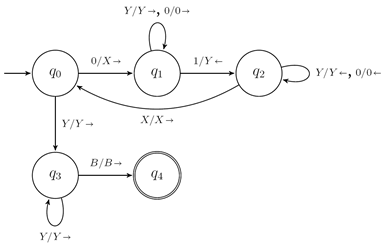
\includegraphics[scale=1.2]{Fig_T.png}
  \caption{Диаграмма переходов машины Тьюринга}\label{stud:fig:1}
\end{figure}


\subsection{Фрагменты исходного кода}

Для иллюстрации излагаемого материала в основной текст можно вставлять фрагменты исходного кода (тексты программ). Они должны быть набраны моноширинным шрифтом (например, \texttt{Courier New}), 12~пунктов, с~одинарным интервалом и выравниванием по левому краю. Если к~фрагментам кода требуется указывать ссылки, их тоже надо снабжать заголовками, как в~случае листингов~\ref{stud-lst:1}--\ref{stud-lst:3}, приведенных ниже.

Если строка кода не помещается на одну строку страницы, её следует разбивать на части в соответствии с принятым стилем форматирования кода, а не автоматически. Размер непрерывных фрагментов исходного кода не должен превышать половины страницы. Фрагменты большего размера следует помещать в приложении к работе.


\subsubsection{Примеры фрагментов кода}

Ниже приведены листинги с заголовками.

\begin{lstlisting}[language=C++, caption={C++, пример кода}, label=stud-lst:1]
#include <iostream>
int main()  // однострочный комментарий
{
  std::cout << "Привет, мир!" << std::endl;
}
\end{lstlisting}


\begin{lstlisting}[language=Python, caption={Python, пример кода}, label=stud-lst:2]
print("Привет, мир!")  # comments
\end{lstlisting}

\begin{lstlisting}[language=TeX, caption=\LaTeX, label=stud-lst:3]
% параметр language в наших листингах только для себя
\bf Привет, мир!
\end{lstlisting}



%=======================
\newpage
\section{Примеры оформления формул}

Внутритекстовая формула
$ \int\limits_a^b f(x)\,dx$ не всегда выглядит красиво даже в \LaTeXe.

Но формулы, вынесенные в отдельную строчку всегда выглядят шикарно
\[
  \lim_{d\to 0} S_n =
  \int\limits_a^b f(x)\,dx.
\]

Для того чтобы {\TeX} автоматически мог ссылаться на нумеруемые формулы нужно указывать команду \verb"\label"
\begin{equation}\label{eq:1}
  \frac{abc}{xyz}.
\end{equation}
Формула (\ref{eq:1}) была оформлена с помощью окружения \textsf{equation}.

%=======================
\newpage
\addcontentsline{toc}{section}{Заключение}
\section*{Заключение}

Как итог, на данный момент создана универсальная рекомендательная система с адаптивным ансамблем моделей, способная к полностью автоматическому переформированию представлений данных, пересозданию и переобучению моделей, способная работать для любого интернет-магазина при условии предоставления им стандартизированной выгрузки данных. На данный момент производится А/B тестирование на серверах интернет-магазинов для определения действительной эффективности системы. \\
Кроме того, текущий результат работы был опубликован на конференции МКО-2022 в виде тезисов и видеопрезентации доклада. [Приложения 1,2]



%=======================
\newpage

\addcontentsline{toc}{section}{Литература}
\renewcommand{\refname}{\centering \textbf{Литература}}

% БИБЛИОГРАФИЯ

\begin{thebibliography}{0}
\bibitem{stud:b0}
Рекомендации по оформлению
и представлению курсовых
и выпускных квалификационных работ
студентов института математики,
механики и компьютерных наук.~--
Ростов н/Д, 2020.

\bibitem{stud:b1}
Жуков М.\,Ю., Ширяева Е.\,В.
\LaTeXe: искусство набора и вёрстки текстов с~формулами.~-- Ростов н/Д : Изд-во ЮФУ, 2009.

\bibitem{ALS:a1}{
	Gábor Takács, Domonkos Tikk,
	Alternating least squares for personalized ranking,
	DOI: 10.1145/2365952.2365972 
}

\bibitem{ALS:a2}{
	Github reporistory of "implicit" library,
	https://github.com/benfred/implicit,
	обр. 2021-12-28,
}

\bibitem{AE:a1}{
	Oleksii Kuchaiev, Boris Ginsburg,
	Training Deep AutoEncoders for Collaborative Filtering,
	https://arxiv.org/pdf/1708.01715.pdf 
}

\bibitem{DRN:a1}{
	Ali Elkahky, Yang Song, Xiaodong He,
	A Multi-View Deep Learning Approach for Cross Domain User Modeling in Recommendation Systems,
	https://www.microsoft.com/en-us/research/wp-content/uploads/2016/02/frp1159-songA.pdf 
}

\end{thebibliography}



\end{document}
% ----------------------------------------------------------------


\lstset{ %
language=Python,                 % выбор языка для подсветки (здесь это С++)
basicstyle=\small\sffamily, % размер и начертание шрифта для подсветки кода
numbers=left,               % где поставить нумерацию строк (слева\справа)
numberstyle=\tiny,           % размер шрифта для номеров строк
stepnumber=1,                   % размер шага между двумя номерами строк
numbersep=5pt,                % как далеко отстоят номера строк от подсвечиваемого кода
backgroundcolor=\color{white}, % цвет фона подсветки - используем \usepackage{color}
showspaces=false,            % показывать или нет пробелы специальными отступами
showstringspaces=false,      % показывать или нет пробелы в строках
showtabs=false,             % показывать или нет табуляцию в строках
frame=single,              % рисовать рамку вокруг кода
tabsize=2,                 % размер табуляции по умолчанию равен 2 пробелам
captionpos=t,              % позиция заголовка вверху [t] или внизу [b]
breaklines=true,           % автоматически переносить строки (да\нет)
breakatwhitespace=false, % переносить строки только если есть пробел
escapeinside={\%*}{*)}   % если нужно добавить комментарии в коде
extendedchars=true,
commentstyle=\color{mygreen},    % comment style
stringstyle=\bf,
commentstyle=\ttfamily\itshape,
keepspaces=true % пробелы между русскими буквами
aboveskip=3mm,
belowskip=3mm

}


\renewcommand\NAT@bibsetnum[1]{\settowidth\labelwidth{\@biblabel{#1}}%
   \setlength{\leftmargin}{\bibindent}\addtolength{\leftmargin}{\dimexpr\labelwidth+\labelsep\relax}%
   \setlength{\itemindent}{-\bibindent+\fivecharsapprox}%
   \setlength{\listparindent}{\itemindent}
\setlength{\itemsep}{\bibsep}\setlength{\parsep}{\z@}%
   \ifNAT@openbib
     \addtolength{\leftmargin}{\bibindent}%
     \setlength{\itemindent}{-\bibindent}%
     \setlength{\listparindent}{\itemindent}%
     \setlength{\parsep}{0pt}%
   \fi
}
\renewcommand{\thesection}{\arabic{section}.}
\renewcommand{\thesubsection}{\arabic{section}.\arabic{subsection}.}
